

\documentclass[11pt,a4paper,titlepage,oneside]{article}

\usepackage[most]{tcolorbox}
\usepackage{geometry}
\usepackage{svg}

\usepackage{hyperref} %links
\usepackage{xurl}

\usepackage[document]{ragged2e} %floating text
\usepackage{helvet} %font
\usepackage{tocloft} % dots in table of contents sections

\usepackage{lipsum, multicol}
\usepackage{fancyhdr}
\usepackage{listings}


% citaitons
\usepackage{natbib}

% hypthenationrules
\usepackage[T1]{fontenc}



%redefine the entire fucking bib environment so we dont have the horisontal spacing
% this was generated entirely by chatgpt

\makeatletter
\renewenvironment{thebibliography}[1]
  {\section{Lähteet}%
   \@mkboth{\MakeUppercase{\refname}}{\MakeUppercase{\refname}}%
   \list{\@biblabel{\@arabic\c@enumiv}}%
        {\settowidth\labelwidth{\@biblabel{#1}}%
         \leftmargin\labelwidth
         \advance\leftmargin\labelsep
         \setlength\itemindent{-\labelwidth}
         \setlength\itemsep{10pt} % Change this value to adjust the space between items
         \@openbib@code
         \usecounter{enumiv}%
         \let\p@enumiv\@empty
         \renewcommand\theenumiv{\@arabic\c@enumiv}}%
   \sloppy
   \clubpenalty4000
   \@clubpenalty \clubpenalty
   \widowpenalty4000%
   \sfcode`\.\@m}
  {\def\@noitemerr
    {\@latex@warning{Empty `thebibliography' environment}}%
   \endlist}
\makeatother





%this is such a shitshow lmao

\hypersetup{
    colorlinks=false,
    citecolor=black,
    filecolor=black,
    linkcolor=black,
    linkbordercolor=1 1 1,
    citebordercolor=1 1 1,
    pdfborderstyle={/S/U/W 1},
    urlbordercolor=0 0 1,
    urlcolor=blue
}
\urlstyle{same}



\geometry{
    a4paper,
    left=3cm,
    right=2.5cm,
    top=3cm,
    bottom=2.5cm
}

%remove random margin on side ? idk what happend
%\setlength{\oddsidemargin}{0pt}



%custom reusable colorbox rules
\newtcolorbox{simplebox}{colback=white, sharp corners, boxrule=1pt }


\renewcommand{\contentsname}{Sisällys} % override Contents => Sisallys on table of contents

\renewcommand{\familydefault}{\sfdefault} % set font

\renewcommand{\cftsecleader}{\cftdotfill{\cftdotsep}} % dots for sections

\renewcommand{\bibsection}{\section{Lähteet}}



\def\filename{src/oppari.tex}



\def\testmode{1}






\newcommand\wordcount{
    \immediate\write18{texcount -sub=section \filename{} -inc  | grep Section | sed -e 's/+.*//' | sed -n \thesection p > 'count.txt'}
(\input{count.txt}words)}


\newcommand{\inputf}[1]{\def\filename{#1}\input{#1}}


\newcommand\filewcount{
    \immediate\write18{texcount -1 -sum \filename{} > count.txt }
    \input{count.txt} words }


% jos on testi definetty niin tee 
\newcommand{\istest}[2]{\ifx\testmode\undefined #2 \else #1 \fi}


% testi section näyttää word countin siltä sectionilta jos ei testi niin sitten näytä vain normaali section
\newcommand{\tsection}[2]{\istest{#1{#2\\} \wordcount \\ \medskip }{#1*{#2}}}


\newcommand{\pagesection}[1]{\istest{\section{#1}  }{\section*{#1}}}
\newcommand{\pagesubsection}[1]{\istest{\subsection{#1}  }{\subsection*{#1}}}


% adds page with everything
\newcommand{\addPage}[2]{
    \def\filename{#1}
    \pagesection{#2}
    \istest{ \filewcount \medskip }{}
    \input{#1}
}



% OPPARI SPESIFIC

\newcommand{\addPageOp}[2]{
    \def\filename{#1}
    \pagesubsection{#2}
    \istest{ \filewcount \medskip }{}
    \input{#1}
}

%lab citation style
\newcommand{\labcite}[1]{\setcitestyle{aysep={},open={(},close={.)}}\citep{#1}{}}

%lab citation style
\newcommand{\labciteend}[1]{\setcitestyle{aysep={},open={(},close={).}}\citep{#1}{}}

\newcommand{\labimgcite}[1]{\setcitestyle{aysep={},open={(},close={)}}\citep{#1}{}}

\newcommand{\hurl}[1]{\href{#1}{{\underline{\textcolor{blue}{#1}}}}}


% counter kuville
\newcounter{imgCounter}
\setcounter{imgCounter}{0}

\newcommand{\getImgCount}{
\addtocounter{imgCounter}{1}
\theimgCounter
}


% counter kaavioille
\newcounter{chartCounter}
\setcounter{chartCounter}{0}

\newcommand{\getChartCount}{
\addtocounter{chartCounter}{1}
\thechartCounter
}



\usepackage[finnish]{babel}
















% ------------------------------ BEGIN DOCUMENT ------------------------------ %
\begin{document}

\pagestyle{empty}


%------------------------------ COVER PAGE ------------------------------ %


\includegraphics[width=5cm,height=1cm]{./src/labimg.jpg}

\vspace{86mm}
\huge
\textbf{Kehityksen seuranta}
\newline

\large

\vspace{5mm}
\textbf{Oppimispäiväkirja}
\normalsize

\vspace{90mm}

LAB-ammattikorkeakoulu \newline
\vspace{2mm}
Tieto-ja tietolikenadsfklj, Insinööri (AMK) \newline
\vspace{2mm}
2024 \newline
\vspace{2mm}
Kimi Malkamäki

\newpage




%------------------------------ FIRST PAGE OF ABSTRACT ------------------------------ %
\begin{tabular}{ | l | }

    %hack for the tiivistelmä line
    \multicolumn{1}{l}{
        \begin{minipage}{6cm}
            \hspace{1mm}
            
        \end{minipage}
        \begin{minipage}{4.25cm}
            \hspace{1mm}
        \end{minipage}
        \begin{minipage}[t][1.95cm][t]{3.62cm}
            \large
            \textbf{ Tiivistelmä }
        \end{minipage}
    }\\

    \hline
    \begin{minipage}[b]{6cm}
        tekijä(t)
        \newline
        kimi malkamäki 
    \end{minipage}%
    % 2x2
    \begin{minipage}{8.5cm}
        \begin{tabular}{ | l | c | }
            \begin{minipage}[t][1cm][t]{4.25cm}
                julkaisun laji
                \newline
                Opinnäytetyö, AMK
            \end{minipage} & %
            %
            \begin{minipage}{3.62cm}
                valmistusaika
                \newline
                2024
            \end{minipage} \\ \hline%
            %
            \begin{minipage}[t][1cm][t]{4.25cm}
                sivumäärä
                \newline 
                xx+xx
            \end{minipage}
            &  \\ \hline
        \end{tabular}
    \end{minipage}%
    % end of 2x2
      \\ \hline

    \begin{minipage}[t][2cm][t]{8cm}
    Työn nimi 
        \newline 
    ammatissa kasvaminen 
        \newline 
    oppimispäiväkirja  
    \end{minipage}\\ \hline

    \begin{minipage}[t][1.5cm][t]{10cm}
    tutkinto ja koulutusala.\newline  tietoviestintätekniikka insinööri amk  

    \end{minipage}\\ \hline

    \begin{minipage}[t][7cm][t]{5cm}
    tiivistelmä: \newline lorem ipsim
    \end{minipage}\\ \hline

    \begin{minipage}[t][2cm][t]{5cm}
    avain sanat
    \end{minipage}\\ \hline

\end{tabular}

\newpage



% ------------------------------ SECOND PAGE OF ABSTRACT ------------------------------ %

tiivistelmä








\newpage


% ------------------------------ TABLE OF CONTENTS ------------------------------ %

%keep page numbers off
\setcounter{page}{0}
\pagestyle{empty}
\pagenumbering{gobble}

\tableofcontents





\newpage



% ------------------------------- TERMISTÖ ------------------------------- %


TERMISTÖ
\bigskip

(tiedän ettei termistö kirjoiteta tällä formaatilla. tämäkin on hyvin kesken)
\bigskip
 
%this needs to be aligned cannot be like this make minipage maybe
ECMAscript = skriptaus-kieli standardi 
\bigskip

VDOM = virtual DOM
\bigskip

Transpilaatio = ohjelmointi keilen kääntäminen toiseen ohjelmointikieleen
\bigskip



\newpage





% ------------------------------- CONTENT PRELUDE COMMANDS ------------------------------- %
%enable page counting
\pagenumbering{arabic}
\clearpage
\setcounter{page}{1}

%set heaader and footer
\pagestyle{fancy}
%%
\lfoot{}
\cfoot{}
\rfoot{}
%%
\lhead{}
\chead{}
\rhead{\thepage}
%%
\renewcommand{\headrulewidth}{0pt}
\renewcommand{\footrulewidth}{0pt}
%\newcommand{\n}{\newline\vspace{20mm}}


\section{Johdanto}              % ------------------------------- JOHDANTO ------------------------------- %


%tuleeko tähän oikeasti preamble itse tekniikan alasta 

% jos tulee niin sitten jotain siitä että web suunnittelu liikkuu nopeaseti ja siellä on kokoajan uusia teknologioita
%mutta pohjalta ne perustuu samoihin periaatteisiin.

% tullaanko tekemään seuranta vai jos tulee tarpeeksi tekstiä niin onko ok vaan tehdä normi oppari tästä
% jos tavoitteena olisis se uuden featuren lisääminen

Opinnäytetyön tavoitteena on seurata kehittymistä 13 viikon seurantajakson aikana työharjoittelussa 
ja tutkia henkilökohtaista kehitystä harjoituksen aikana.
%more text
\medskip


opinnäite työ on päiväkirjamallinen ja liitteenä on päiväkirja dokumentti, 
johon olen kirjannut mitä olen tehnyt, mitä olen oppinut ja minkälaisten teknologioiden kanssa olen ollut tekemisissä.
%more text
\medskip


Työ toteutettiin Starttaamo Oy:ssä. Starttaamo on suomalainen startup yritys, joka pyrkii ratkomaan ongelmia työergonomian kanssa.
startupin pää tavoitteena on vähentää sairaslomia saamalla työntekijät noudattamaan, alojen ammattilaisten suunnittelemien liikunta- ja ruokavalio-ohjelmia. 
Yrityksen pää myyntituote on web-alusta. (jotain lisäää tekstiä)
%more text
\medskip






\newpage
\section{Lähtötilanne}         % ------------------------------- LÄHTÖTILANNE ------------------------------- %


Ennen opinnäytetyön kirjoittamista ja seurantajakson alkamista. 
% kauan olen ollut opiskelija
Olin opiskellut LAB ammattikorkeakoulussa XX lukukautta ja olen opinnäytetyön kirjoituksen aikana neljännen vuoden tieto- ja tietoviestintätekniikkan opiskelia.
% jotain lorem siitä että olen oppinut koulusssa jotain
%
% jotain siitä että ei ole oikeaa työ kokemusta vaikka on vahva koodauspohja
Minulla ei ennen harjoitusta ollut aijempaa työkokemusta alalta, (joten jotain jotain jotain).
\medskip







\newpage
\section{Teoria}                % ------------------------------- TEORIA ------------------------------- %



\subsection{Kehitys ympäristö / Teknologia pino}

% tässä voisi yleisesti kertoa miksi nämä teknologiat on valittu tai on käytössä.. alempana kuitenkin kerrotaan mitä ne on ja miten toimmii

Startupit haluaa nopeaa liikkumista ja kehittymistä ja se näkyy teknologioiden valinnassa.
Projekti käyttää Meteor fullstack frameworkkia, joka on suunniteltu nopeaan kehittämiseen ja käyttöönottoon.
%more text
\medskip

Käyttöliittymä on toteutettu käyttämällä reactjs kirjastoa.
%more text
\medskip

projektin tietokanta on mongodb, joka tekee uusien collectioneiden tekemisestä helppoa sillä nosql kantoihin ei travitse määritellä skeemaa.
%more text
\medskip

meteor mongo ja react on core teknologiat jota projekti käyttää mutta mukana on myös pienempiä teknologioita joita opinnäytetyö käy läpi.
yhdessä näitä kolmea teknologiaa käytten voi luoda monenlaisia nopeuta ja skaalautuvia nettisivuja pienistä projekteista suuriin.
%more text
\medskip









\newpage
\subsection{Meteor}                % ------------------------------- Meteor ------------------------------- %



\subsubsection{meteor yleisesti}


%https://github.com/mongodb/mongo?tab=License-1-ov-file
% mongo licence 

% https://github.com/meteor/meteor?tab=License-1-ov-file
% meteor lisence

% https://guide.meteor.com/collections.html#mongo-collections
% meteor uses mongo. but it is not manditory



%tässä blokissa on tarpeeks tekstiä kuhan sen kirjottaa kunnoll


%src meteor homepagef
Meteor on full-stack JavaScript web-framework ja on itsessään avoimeen lähdekkoodiin perustuva, 
poislukien meteorin mukaan paketoimaa mongodb tietokantaa, joka toimii Server Side Public Lisenssillä.
Meteor on suunniteltu nopeaan kehittämiseen monelle laitteille ja nopeaan käyttöönottoon.
%
% https://www.meteor.com/
% viitattu 28.5 ...
% pakota ... frontend teknologiaa ... kehittäjää? mahdollisesti ei tätä edes kun mmeillä on alempana toi featuret
%Meteor ei pakota kehittäjää käyttämään tiettyä front-end teknologiaa vaan sillä on integraatio moneen yleiseen frontend-framework:kiin, kuten Vue, React, Svelte tai Angular.
\medskip

jotain siitä että meteori käynnistää oman backendin ja se käyttää ihan samallaista koodia kun client.
tää tekee clientin ja backendin koodista samanlaisen joka helpottaa käyttöönottoa ja devaamista.
\medskip

    
% https://www.meteor.com/
% viitattu 28.5

Meteor tukee monta ominaisuutta kuten.
\begin{itemize}
    \item Tukee monta Front-end kirjastoa ja frameworkkkia
    \item Tukee Typescriptiä
    \item Sisään rakennettu käyttäjä systeemi
    \item Toimii monella laitteella
    \item Helppo ja nopea käyttöönottaa 
\end{itemize}





\subsubsection{Meteor metodit}

% kirjoita tämä oikeella oppari tyylillä. idk tuntuu vähän väärältä tässä


% kappale rpc. mikä on ja miten eroaa restful

%enemmän yleis selostusta rps ja restful mikä on ero hyvät ja huonot puolet

Meteor ei käytä RESTful rajapintaa vain RPC (eng Remote procedure call) rajapintaa. 
%uusiks
Tarkoittaa että client kutsuu funktioita palvelimella meteorin kautta.
%uusiks jotenkin huono 
Palvelimelle määritetään metodit, joita voidaan kutsua palvelimelta tai clientiltä.
\medskip


% ehk uusiks
Methodit suoritetaan ja määritetään funktioina palvelimen puolella, ja niitä voi kutsua clientistä tai palvelimelta.
% uusiks ainakin alku. 
Metodit antavat kutsujasta tietoa, esim. onko kutsuja kirjautunut sisään ja jos on niin mikä on hänen käyttäjätunnuksensa. 
%uusiks
Näin voi helposti katsoa onko kutsujalla tai käyttäjällä oikeuksia metodin kutsumiseen.
\medskip




\subsubsection{Meteor ecosysteemi}
meteor package management system ja meteorin deploy systeemit (galaxy etc)








\newpage
\addPageOp{./src/op/react.tex}{React}% ------------------------------- REACT ------------------------------- %






\newpage
\addPageOp{./src/op/mongo.tex}{Mongodb}        % ------------------------------- MONGODB ------------------------------- %











\newpage
\subsection{Responsiiviset käyttöliittymät}

\subsubsection{Responsiivisten käyttöliittymien suunnittelun periaatteet}

WORK IN PROGRESS LOREM FOR RESPONSIIVINEN
\medskip


% kirjoita eritavalla ettei oo copypasta
Responsiivinen verkkosuunnittelu on lähestymistapa verkkosivustojen rakentamiseen, jolla varmistetaan niiden optimaalinen ulkoasu ja toimivuus eri laitteilla ja näytön koossa.
Käyttämällä responsiivisia verkkosuunnittelua verkkosivustot voivat tarjota yhdenmukaisen käyttökokemuksen eri laitteilla.

idea on tehdä verkkosivu jota voi käyttää eri laitteilla, jolla on eri näytönkoot
\medskip


% uudelleen kirjoita jotankin että sama asia mutta ei copypasta kuitenkaan päiväkirjasta
Web-käyttöliittymissä elementtien koot voivat olla absoluuttiset tai suhteelliset niiden ylempään elementtiin verrattuna. Absoluuttiset arvot tarkoittavat, että elementti olisi aina tietyn kokoinen pikseleissä. 
Tämä voi luoda tilanteita, jossa pienempikokoisemman näytöllä joku elementti on liian iso, tai ei sovi enää käyttöliittymään, joten absoluuttisia ei voi käyttää responsiivisessa käyttöliitymässä.
% asiakielellä. eivät kuitenkaan ei kuulosta oikeelta jutulta
Relatiiviset elementtikoot eivät kuitenkaan ratkaise kaikkia ongelmia. Mobiili- ja työpöytälaitteiden kuvasuhteet eroavat. Käyttöliittymän pitää olla erilainen jos pituutta on enemmän, kun leveyttä. 
Ja, koska työpöytälaitteita käytetään hiirellä, joka antaa tarkan osoittimen käyttäjälle, toisin kuin mobiilissa, jota käytetään sormilla. 
Pitää ottaa huomioon linkkien, nappien ja kuvakkeiden koko, jotta itse sovelluksen käyttäminen olisi huoletonta.\medskip
\medskip




\subsubsection{Css Mediaquery}

lorem ipsum

lorem ipsum






\newpage
\subsection{Web sivustojen kääntäminen}

% sana lokalisaatio pitäisi vaihtaa translaatioksi
% sillä me emme tehnyt mitään oikeaa lokalisaatiota


%link tree
% https://www.linkedin.com/pulse/website-translation-how-to-guide-louise-souter


% people prefer content in their lenguage
%https://csa-research.com/Featured-Content/For-Global-Enterprises/Global-Growth/CRWB-Series/CRWB-B2C#10Facts
% 11.6


%kääntäminen yleisesti ja miksi sen tekisi. ja jotain itse lokalisaatiosta

Kielimuuri on iso ongelma tuotteiden ja nettisivujen laajentamisessa uusille markkinoille.
% uusiks
csa rechearching väittää että 65\% käyttäjistä suosisi sisältöä heidän kielellä.
\medskip





%https://www.transifex.com/blog/2024/website-translation-methods/
%11.6 

On monta eri menetelmää sivustojen kääntämiseen, 
ja koska monet kielet on hyvin erillaisia voi konteksti ja nuanssi hävitä jos kääntää vain sana sana sanaan.
Monet lausahdukset ja sanonnat ei voi kääntää suoraan kielestä toiseen ilman että menettää sen alkuperäisen tarkoituksen.
esimerkiksi (joku esimerkki sanonnasta joka ei toimi jos sen kääntää englanniksi).
\medskip


%add more words to this
Käännös teksin luonnin voi yleisesti tehdä kahdellla tavalla. Ihmis käännös tai tekoälykäännös.
Ihmis käännöksellä voi olla hyvä tarkkuus ja lopputulos tulee kuulostamaan luonnolliselta.
tekoaly käännös on tosi nopea, mutta ei vielä ole tarpeeksi tarkka kaikkiin käyttötarkoituksiin.
\medskip




%https://www.motionpoint.com/platform/what-are-the-best-technologies-for-website-translation/
% 11.6


On eritapoja toteuttaa käännösten tekeminen web alustoilla. Monet suuret sivustot kutem amazon \citemissing{} 
hostaa monta eri versiota niiden nettisivuista.
legit hard kopio nettisivusta joka on kirjoitettu eri kielellä. Tämä on hyvin kallis ja aikaavievä.

Tekstin Hot swappaaminen. Käytetään yhtä sivua mutta teksti vaihtuu alta kun vahdetaan kieli. \citemissing{}
käytetään jotain keskitettyä kielipankkia johon kaikki käännökset on tallennettuna.
\medskip


Hot swappaamisessa...\\
Kovakoodatut tekstit sivuilta vaihdetaan käännösfunktiokutsuihin.
Funktio etsii käännöstiedostosta oikeat sanat tai lauseet ja asettaa ne alkuperäisen tekstin tilalle. 
Käännöstiedost on avain-arvo. %jotain tähän vielä
% asiakielellä uusiks
Avain on valmiiksi päätelty merkkijono ja arvo on itse käännös. 
Kun haluttu kieli vaihdetaan kirjasto vaihtaa käännöstiedoston toiseen tiedostoon jolla on samat avaimet. 
Arvot vain vaihtuvat uuden kielen tekstiksi.\citemissing
\medskip












\newpage
% mahdollissesti toteutus title pois että saa yhden lisää subsectiionin muuten tää on vähän liikaa alalukuja

\section{Käännösten toteutus}

\subsection{wip title tehtävä}
Sovelluksen sivut on kovakoodattu suomeksi. ja ne pitäisi pitäisi pystyä kääntämään.
\medskip


\subsection{Käytetty teknologia}
Meteorin kanssa yhteensopiva i18n kirjastoa käyttäen käännöksien luonti ei ole monimutkaista.
Kaikkien julkisesti olevien teksien etsiminen ja vaihtaminen i18n käännös funktio kutsuihin.
Käännös tiedoston luominen ja käännöksien laittaminen.
\medskip
\bigskip


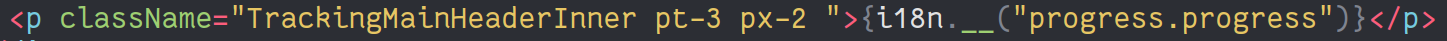
\includegraphics[width = 15cm]{src/public/oppar/translationcall.png}\\
Kuva \getImgCount. {} i18n käännösfunktiokutsu (ehkä uusi kuva)
\medskip

kuvassa luodaan HTML paragraafi elementti jossa kutsutaan käännösfunktiota. funktio hakee käännöstiedoston progress sivulta progress arvon.
\bigskip


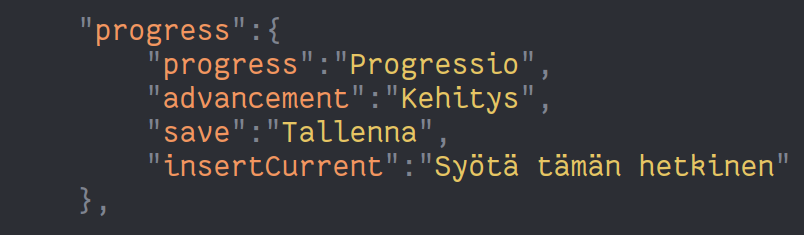
\includegraphics[width = 15cm]{src/public/oppar/translationfile.png}\\
Kuva \getImgCount. {} progressiosivun käännökset suomenkieliseltä käännöstiedostosta(ehkä uusi kuva)
\medskip

kuvassa progressio sivun käännökset. käännös tiedoston on json formaatissa joten sivut ovat omia objekteja. 
niiden ominaisuudet ovat avaimia mitä käytetään kun haetaan käännöksiä ja arvot ovat julkinen teksi.
Kuvassa \nextImageCount {} On Sama kohta käännöstiedostosta mutta englannin kielisestä
\medskip
\bigskip


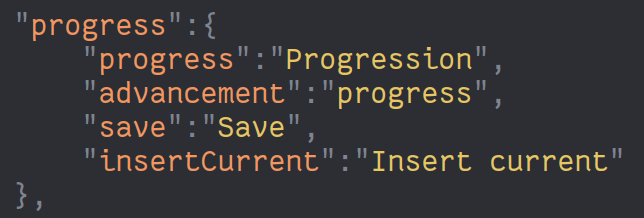
\includegraphics[width = 15cm]{src/public/oppar/translationfileEng.png}\\
Kuva \getImgCount. {} progressiosivun käännökset englanninkielisestä käännöstiedostosta(ehkä uusi kuva)
\medskip

\subsection{käyttöliittymä kielenvaihamiselle}

laskuvalikko kun vaihdetaan kieli


\subsection{wip title kaksi}
Sovelluksen kaikki julkisesti oleva teksi on siirretty käännös tiedostoihin. 
Tämä luo keskitetyn sijainnin josta voi helposti etsiä ja korjata kirjoitus virheitä ja lisäämään uusia lauseita ja sanoja.
uuden kielen lisääminen vaatii uuden käännöstiedoston luomisen ja käännös arvojen asettelun tiedostoon.
\medskip

% saadaanko jotain lisää kirjoitettua ns "yhteenvetoon"













\newpage
\section{Uuden ominaisuuden lisäys}

\subsection{Alkuperäinen ominaisuus ja parannus kohteet}
progressio sivy ja measurable thing joka on user skeemassa vain yksi juttu
tämä pitää tehdä jotain että kaiikki on hybää
\medskip

kuva sivulta

selitys mitä sivulla tapahtuu
\medskip

kuva nykyisestä skeemasta

selitys skeemasta ja miten se liittyy sivuun
käyttäjän profiilissa on ominaisuus measurableThing. tätä käyttäen sovellus tietää mitä arvoa mitataan.
Yksittäinen measurableThing ei riitä jos halutaan mitata useampaa arvoa.
itse tietokannassa on oma mongo collection progressio arvoille jossa mitattava arvo on nimetty merkkijonona.
tätä ei tarvitse muokata sillä voimme vain etsiä mitä tietoja halutaan mongo queryillä.
\medskip



\subsection{Ominaisuuden totetus}

user skeeman muutos ja migraatio


tarvittavat muutokset skeeman muutoksen jälkeen. rajapinta muutokset jne (ei olla selitetty gql joten siitä ei paljoa)


käyttäjän luonti ja käyttäjän päivittämis apin muokkaaminen.
mittatuloksien laittamimnen api

kuva käyttäjä luomis interface before and after


käyttöjän datan laittamis userinterface
toinen kuva uudesta käyttöliittymästä


\subsection{Ominaisuuden lopputulos ja käyttöönotto}
migrate meni hyvin. tosin jos olisi ottanut backupin databasesta niin ei olisi ollut riskiä hajottaa kaikkea.
\medskip

itse feature toimi hyvin käyttöön oton jälkeen ja kaikki käyttäjät saivat ominaisuuden käyttöön
\medskip

käyttöliittymästän toiminnasta tai sen ulkonäöstä ei tullut palautetta senjälkeen kun se oltiin käyttöön otettu joten sekin meni hyvin.
\medskip












\newpage
\section{Yhteenveto}

sehän meni ihan hyvin 

opin käyttämään projektissa käytettyjä teknologioita
opin tekemään töitä ammatillisessa työympäristössä
\medskip


lokalisaatio meni hyvin ja sovellus on nyt parempi
\medskip


uusi ominaisuus toimii ja siitä ei tullut ognemlia sen käyttöönotossa
\medskip





\newpage

% we need some way to manually override an item when it looks like shit

% i thin we need to make our own @ thing then use that for htings that look like shit
% though i dont thik we need the hfill thing in the first place but whattever that is problem for another day


(korjaa outo spacing)
\bibliographystyle{labCitations} % ------------------------------- LÄHTEET ------------------------------- %
\bibliography{./src/op/citations}


%https://libguides.eur.nl/overleaf/bibliographies-and-citing
%https://tex.stackexchange.com/questions/51434/biblatex-citation-order
% i want to do citations like this but if there is problem with the format then must do manually or... write own system





\section{Liitteet}               % ------------------------------- Liitteet ------------------------------- %

miten laitan liitteen päiväkirjasta ja millainen se pitäisi olla








\end{document}
